\documentclass[12pt,a4paper]{article}

% ---------- Page layout ----------
\usepackage[a4paper,margin=2.5cm]{geometry}
\usepackage{setspace}
\onehalfspacing
\setlength{\parindent}{0pt}
\setlength{\parskip}{0.75em}
% Let TeX stretch interword space a little further before it gives up and
% pushes a line into the margin. Without this the long BigQuery table names
% and index tickers produce overfull lines.
\setlength{\emergencystretch}{3em}

% ---------- Tables and figures ----------
\usepackage{graphicx}
\graphicspath{{figures/}}
\usepackage{booktabs}
\usepackage{threeparttable}
\usepackage{caption}
\usepackage{float}
\usepackage{array}
\usepackage{tabularx}
\usepackage{eurosym}

% ---------- Math and symbols ----------
\usepackage{amsmath}
\usepackage{amssymb}

% Wide tables are set one step down and with tighter column padding, so that
% they fit the text block instead of running into the margin. Applied inside
% threeparttable, this narrows the table notes to match.
\newcommand{\compact}{\setlength{\tabcolsep}{3.5pt}\small}
\newcommand{\compactx}{\setlength{\tabcolsep}{3pt}\footnotesize}

% ---------- References ----------
\usepackage[round,authoryear]{natbib}
\bibliographystyle{apalike}

% ---------- Links ----------
\usepackage{xcolor}
\usepackage[colorlinks=true,linkcolor=black,citecolor=blue,urlcolor=blue]{hyperref}

% ---------- Thesis metadata ----------
\newcommand{\thesistitle}{Whose Perception of Geopolitical Risk Is Priced in Defence Equities?\\[0.4em]Evidence from the Russia--Ukraine War}
\newcommand{\thesisauthor}{Khrystyna Kateryna Valenia}
\newcommand{\thesisdate}{August 2026}

\begin{document}

%--------------------------------------------------------------
\begin{titlepage}
  \centering
  \vspace*{2cm}
  {\LARGE\thesistitle\par}
  \vspace{1cm}
  {\large \thesisauthor\par}
  \vspace{0.5cm}
  {\large \thesisdate\par}
  \vspace{1cm}
  \begin{abstract}
  \noindent
  Every standard measure of geopolitical risk is built from English-language newspapers. This thesis asks whether that editorial vantage point is the one that matters for defence-equity prices, or whether local-language perception --- from Ukrainian and Russian outlets, closer to the conflict --- carries additional information. Using 4,027 days of multilingual news data from GDELT's translingual archive, classified by the publisher's national identity rather than by article subject, this thesis tests whether Ukrainian, Russian state, and Russian independent coverage of the Russia--Ukraine war explains defence-equity returns conditional on Western coverage already being in the regression. The answer is no. Local perception adds nothing in coverage volume, in tone, or in the structure of anticipatory versus realised reporting, across two asset classes (defence equities and European natural gas) and one non-market outcome (realised escalation). A power simulation on 1,855 out-of-sample days confirms the test would detect an effect of 0.5\% out-of-sample R$^2$ in roughly five simulated samples out of six: the range the literature treats as economically meaningful is ruled out. Russian state media's tone did not move when Russia invaded Ukraine ($+0.02$); Ukrainian media's tone fell by 1.66 points. Markets track one of those two signals.
  \end{abstract}
\end{titlepage}

\newpage
\tableofcontents
\newpage

%==============================================================
\section{Introduction}
%==============================================================

The Russia--Ukraine war is the most intensively covered armed conflict in modern media history, and it produced the sharpest repricing of defence equities in decades. European defence equities rose 21.6\% in the five weeks following the 24 February 2022 invasion, against 7.0\% for the global sector index and 9.1\% for its U.S.\ counterpart; the sector then re-rated far more dramatically in the first half of 2025 (Europe $+63.7$\%) as European governments announced rearmament budgets. For an investor trying to understand that repricing, the natural question is: what information is driving it? The standard answer in the geopolitical-risk literature is ``what newspapers say'' --- but which newspapers? The two most widely used indices, those of \citet{caldara2022} and \citet{baker2016}, are built from a fixed panel of English-language, mostly American and British outlets. When a defence-equity price is said to be responding to geopolitical risk, it is responding to a quantity constructed from one particular editorial perspective --- the Western one.

\textbf{The research question of this thesis is: whose perception of geopolitical risk is priced in defence equities?} Two candidate answers are possible. Either the information that moves defence-equity prices originates where the war is fought --- in Ukrainian and Russian media, which are closer to the battlefield, cover it more intensively, and carry it earlier --- and reaches Western prices with the delay that translation and attention impose. Or Western markets price the Western narrative, and local coverage, however earlier or more voluminous, adds nothing once the Western signal is controlled for.

\textbf{The first challenge is measurement.} The submitted version of this project built Ukrainian, Russian, and Western sentiment series from GDELT's Global Knowledge Graph version 1.0 --- a stream that is effectively English-only (7 articles from \texttt{.ru} domains out of 60,690 in a typical day), in which nationality was assigned by the country an article \textit{mentioned}, not by the country that published it. The series labelled Ukrainian and Russian sentiment were, in practice, English-language articles about Ukraine and Russia: one population sorted by topic and relabelled as three perspectives. This makes the source-group comparison meaningless. The correction is to use GDELT's \textit{translingual} archive, which processes material in 65 source languages and classifies each article by the outlet that published it, providing genuine Ukrainian and Russian media signals. The rebuilt indices run from 18 February 2015, when the translingual archive begins, and cover 4,027 calendar days.

\textbf{The second challenge is identification.} News coverage of a conflict and defence-equity prices may move together for many reasons that have nothing to do with the media ecosystem carrying the signal. Both respond to the same underlying events; financial market conditions affect both; and a common regime trend contaminates any level regression. The strategy addresses this through a conditional joint F-test: local media are asked whether they add to returns \textit{conditional on Western coverage already being in the regression}. This mirrors the test in \citet{bondarenko2024}: they ask whether local Russian risk measures add to English-language measures for the Russian economy; this thesis asks the same question for the counterparty's assets. Because the correct market control for European defence equities is a European index (not the S\&P 500, which was used in the submitted version), the analysis uses STOXX 600 returns as the market control, which eliminates an artefactual result documented in Section~\ref{sec:robustness}.

\textbf{The third challenge is multiple testing.} The specification grid crosses frequency (daily, weekly), episode window (six anticipation periods plus the full sample), and five defence-equity targets, producing 31 testable cells. Running 31 tests at 5\% significance would yield roughly 1.5 false rejections by chance. The analysis applies Benjamini--Hochberg correction across the full grid and, for the anticipation-structure test (Gate 3), pre-registers the pass rule, the excluded targets, and the sign condition before building the test. Gates 4 and 5 each have their data ingested after the pre-registration is written. This sequence is verifiable from repository commit history.

\textbf{The fourth challenge is evaluating a null result.} A finding that nothing predicts is worthless unless the reader knows what could have been found. The out-of-sample section of this thesis therefore accompanies its zero Clark--West rejections with a power simulation: using the actual return series and implanting a predictor with a known true effect, the design is shown to detect an out-of-sample R$^2$ of 0.5\% in 83\% of simulated samples and one of 1.0\% in every simulated sample, on 1,855 out-of-sample days. The range of effect sizes the predictability literature treats as economically meaningful is therefore ruled out rather than merely unobserved.

\textbf{Local-language perception adds nothing to defence-equity returns once Western coverage is in the regression, and the design is demonstrably able to detect media effects where they exist.} That second clause is what makes the first one a finding rather than an absence, and it is established test by test rather than in summary: the Western block survives multiple-testing correction in the pre-registered anticipation gate (2 of 31 cells, minimum $p = 0.0002$), in the gas test ($p = 0.001$) and in the escalation test ($p = 0.006$). In the attention-and-tone gate the Western block does not survive correction under the tradeable one-day lag either; what demonstrates sensitivity there is the local block's own behaviour, which is detected on the day of publication and collapses when the news is lagged by the one day that would have made it tradeable. Second, the descriptive evidence reveals a striking asymmetry: Russian state media's conflict tone did not move when Russia invaded Ukraine (aggregate shift: $+0.02$; fixed-outlet panel of 24 state outlets: $-0.05$), while Ukrainian media's tone fell by 1.66 points on the same scale. This asymmetry is both the most interesting empirical fact in the data and consistent with the null finding about pricing: the information set that changed most sharply at the invasion is not the one that markets track. Third, across 50 out-of-sample forecasting specifications, the Clark--West test rejects zero times against 2.5 expected by chance, and simulation confirms this is not a power failure.

\textbf{The primary contribution is to the literature on whose information is priced in financial markets.} \citet{bondarenko2024} show that for the Russian domestic economy, local Russian-language risk perception matters and English-language perception does not. This thesis runs the mirror of that test on the counterparty's assets and finds the reverse asymmetry: Western defence equities price the Western narrative, and the local narrative is redundant once the Western one is controlled for. Neither result licenses a general claim that local media always matter or never matter. Read together they say something more specific and more useful --- that each market prices the information ecosystem its own marginal investors inhabit --- and that claim requires both halves of the mirror to state.

\textbf{The second contribution is to the literature that measures risk from newspaper text, where the question of \textit{which} newspapers has been left largely unexamined.} Since \citet{baker2016} and \citet{caldara2022} established normalised newspaper counts as a workable proxy for uncertainty and geopolitical risk, the resulting indices have been treated as measurements of a latent state of the world rather than as measurements taken from a particular vantage point. This thesis makes the vantage point itself the object of study, and shows that the choice is empirically consequential in one direction and not in the other: the Western vantage point carries the pricing information, and adding three further vantage points to it adds nothing that survives correction.

\textbf{The third contribution is methodological, and concerns how easily this class of measurement goes wrong.} \citet{loughran2011textual} caution that automated sentiment dictionaries require domain-specific validation, which is why GDELT tone is interpreted here as an indicator of coverage negativity rather than as a direct measure of investor beliefs. The submitted version of this project illustrates the same warning at the level of the corpus rather than the dictionary: it measured Ukrainian and Russian sentiment from a stream that is effectively English-only, so that what was labelled provenance was in fact topic. The measurement error was not small, it was not visible in the output series, and it was found only by writing the methodology section out in full. Section~\ref{sec:robustness} reports five further results that were significant when found and did not survive; that sequence is reported rather than suppressed because it is the most transferable thing the project produced.

\textbf{The fourth contribution is to the empirical literature on defence equities and conflict.} \citet{apergis2018defense}, \citet{zhang2022race}, \citet{covachev2024europe} and \citet{klomp2025hamas} establish that defence equities respond to geopolitical events around armed conflicts, and \citet{tetlock2007media} and \citet{manela2017} establish more generally that media content carries information for asset prices at short and long horizons respectively. What this literature aggregates is news; what it does not do is separate news by the nationality of the outlet that produced it. This thesis performs that separation and locates the response in the Western layer specifically.

\textbf{Why this should matter to a reader who is not studying this war.} Practitioners increasingly buy geopolitical-risk signals built from multilingual news feeds on the premise that sources closer to an event are more informative about it. That premise is testable, and in the setting most favourable to it --- an eleven-year sample, the most heavily covered conflict in modern history, an asset class whose investment case is a claim about that conflict, and local media operating at near-saturation coverage --- it does not hold at a horizon a trader could act on. The information that is closer to the event is not thereby closer to the price.

%==============================================================
\section{Data and Identification Strategy}
\label{sec:data}
%==============================================================

\subsection{The news corpus and its construction}

The analysis rests on a corpus of 4,027 days of conflict-related news from GDELT's Translingual Global Knowledge Graph, covering 18 February 2015 (the first day of the translingual archive) to 20 May 2026. The corpus is accessed through BigQuery's \texttt{gdelt-bq.gdeltv2.\allowbreak{}gkg\_partitioned} table, a day-partitioned store of GDELT's global news annotations running to several terabytes, from which only the columns and days required are scanned. An article enters the sample if it geolocates to Ukraine or Russia according to GDELT's country codes. GDELT's translingual stream processes text in 65 source languages, machine-translates it, and applies a unified annotation pipeline, making it possible to compare Ukrainian, Russian, and Western outlets through a single measurement framework.

Each article is assigned to one of five media ecosystems based on the outlet that published it --- not based on the country the article discusses. This distinction is critical: an article in a British newspaper about Russian troop movements is Western, not Russian. The assignment uses four tiers in priority order. First, a hand-curated register assigns high-volume outlets manually, verified by country of registration and editorial ownership. Second, outlets with a nationally registered domain suffix (\texttt{.ua}, \texttt{.ru}, \texttt{.de}, etc.) are assigned by ccTLD. Third, source language is used conditional on GDELT country information. Fourth, unresolved articles fall to a residual ``other'' category. Country of publication takes priority over article language at every tier: Ukrainian outlets publish heavily in Russian (e.g.\ \texttt{24tv.ua} carries 2,595 Ukrainian-language and 1,865 Russian-language articles), and classifying them by language would file those articles as Russian and manufacture agreement between two ecosystems the design needs to keep apart. One further rule is stated because it points in both directions: state-funded external broadcasters classify to the funding state, which puts Deutsche Welle and Radio Free Europe/Radio Liberty in the Western block, while exile newsrooms classify to their country of origin, which keeps \textit{Meduza} in the Russian independent one. Three outlets were misfiled before that rule was written down, and Section~\ref{sec:robustness} reports what one of them cost.

The five resulting ecosystems are: \textbf{UA} (Ukrainian outlets), \textbf{RU\_STATE} (Russian state-controlled), \textbf{RU\_INDEP} (Russian independent), \textbf{WEST} (EU, UK, US, Canada, Australia), and \textbf{EN\_GLOBAL} (English-language global sources). Russian state outlets are identified through ownership registers following the press-freedom classification in \citet{bondarenko2024}. Russian independent outlets include platforms exiled or blocked in Russia such as \textit{Meduza} and \textit{TV Rain}.

\textbf{The register is validated against an external source rather than asserted.} Each registered domain is resolved against Wikidata and its recorded country of origin compared with the assigned ecosystem: of 84 registered outlets, 66 resolve to a verifiable country, and 63 of those agree, a precision of \textbf{0.955}. The Russian state, Western and Ukrainian blocks agree perfectly (1.000 each); all three disagreements fall in the Russian independent block (0.750), and all three are exile newsrooms, which is the one case where country of origin and country of operation genuinely differ. This audit validates that each registered domain belongs to the country it was assigned to. It does not validate GDELT's attribution of a given article \textit{to} a domain, which is taken on trust and would require a reader with Russian and Ukrainian to check.

\textbf{The classification rule is also varied, to establish that the results are not an artefact of it.} Five rules are run through the full test grid: the baseline, a register-only rule that drops the ccTLD and language tiers, a rule with no language tier, a language-first rule, and one that retains news aggregators. The local-block verdict is unchanged under all five --- one or two survivors of 31 cells under the primary alignment in every variant. The language-first rule is the informative failure: because the language tier claims Russian-language articles before ownership is consulted, it cannot represent a Russian independent block at all, which is the concrete cost of the country-before-language rule being got wrong.

\subsection{Perception indices}

Two indices are constructed for each ecosystem per day. The \textbf{attention share} is the count of conflict articles in the ecosystem divided by that ecosystem's total article count, expressed as a percentage. Using a share rather than a raw count is standard practice \citep{baker2016} because the overall size of the GDELT corpus drifts over time. The \textbf{conflict tone} is the mean GDELT tone score for conflict articles in that ecosystem. GDELT tone is a dictionary-based measure ranging from approximately $-10$ (highly negative) to $+10$ (highly positive).

Both indices are used in daily first differences in all regressions. The reason is empirical: in levels, all series carry a common ``war regime'' trend that financial controls already capture, and it is the day-to-day \textit{innovation} in perceived risk, not its persistent level, that should carry price-relevant information. The first-difference transformation is also what \citet{bondarenko2024} apply.

Following \citet{caldara2022}, each ecosystem's attention share is further decomposed into an \textbf{anticipatory component} (articles classified by GDELT's Themes field as covering threats, build-ups, or pre-war events) and a \textbf{realised component} (articles covering acts of war, escalation, or attacks). This threat/act split is the object of the anticipation test in Section~\ref{sec:gate3}.

\subsection{Financial targets and controls}

The primary financial targets are two official Bloomberg defence-equity indices: the Bloomberg World Large, Mid and Small Aerospace \& Defense Total Return Index (\textbf{WAERLST}, USD) and the Bloomberg Europe Defense Select Total Return Index (\textbf{BSHIELDT}, EUR), both running from 2 January 2020 to 29 June 2026 (1,619 trading days, no missing observations). Three further targets extend coverage backwards and separate the two regions, giving five in total: the iShares U.S.\ Aerospace \& Defense ETF (\textbf{ITA}), available for the whole 2015--2026 window and so covering the pre-war baseline the Bloomberg indices miss; and two hand-built equal-weighted baskets of listed defence names, one European (\textbf{EU basket}) and one American (\textbf{US basket}), which extend the same coverage to constituents rather than index vehicles. The two baskets are constructed from free data and are the targets the Gate 3 pre-registration excluded from its primary arm, precisely because they are hand-built.

\textbf{The choice of market control is not a detail; it is the single specification decision that most changed this project's results.} A previous version used the S\&P 500 to control for market movements in \textit{European} defence returns. Over the build-up window the SPX--STOXX 600 correlation is only 0.409, so that choice left a large amount of ordinary European market variation sitting in the residual --- and that residual correlates 0.26 with the threat shock being tested. Two apparently strong findings came out of that gap, and both disappeared when the control was corrected (Section~\ref{sec:robustness}). Every regression here therefore uses the regional market return appropriate to its target: STOXX 600 for European targets, S\&P 500 for global and U.S.\ ones. The remaining controls are the VIX, to absorb general risk appetite, and lagged defence-equity returns, to absorb own-momentum.

\subsection{Physical attack data (supplementary context)}
\label{sec:attacks}

The analysis is grounded in media perception rather than physical events, but a parallel dataset records the physical dimension of the conflict: daily Ukrainian Air Force records of Russian air attacks from 29 September 2022 to 21 June 2026. The raw file contains 3,812 attack-level records, aggregated to 809 unique market-information dates using the rule
\begin{equation}
\text{market\_info\_date} = \max(\text{attack\_date},\; \text{time\_end\_date}),
\end{equation}
which assigns each attack to the day on which the verified count could plausibly enter the market's information set, avoiding look-ahead bias. Across all records, 102,396 weapons were launched and 76,126 were intercepted or destroyed (interception rate: 74.3\%); UAVs account for 94.8\% of all launched weapons. War intensity is measured as $\ln(1 + \text{weapons launched}_t)$.

This dataset is used in two ways. First, it provides physical context for the media patterns in Section~\ref{sec:descriptive}: Western news attention spikes on high-intensity attack days, while local attention is already near saturation. Second, it serves as a robustness control in Section~\ref{sec:robustness}: conditioning the main specification on contemporaneous attack intensity leaves the local-block null unchanged.

The dataset binds the joint sample to September 2022 onward, which is why the primary analysis uses GDELT-only over the longer 2015--2026 window. The physical and perceptual dimensions of the conflict are thus separated in the sample design rather than conflated.

\subsection{Identification strategy}
\label{sec:identification}

The core test asks whether local media add explanatory power to defence returns \textit{conditional on} the Western signal. The specification for each cell in the grid is:
\begin{equation}
r_{i,t} = \alpha + \beta_{\mathrm{West}} \mathbf{X}^{\mathrm{West}}_t + \beta_{\mathrm{Local}} \mathbf{X}^{\mathrm{Local}}_t + \gamma Z_t + \varepsilon_{i,t},
\label{eq:main}
\end{equation}
where $r_{i,t}$ is the return on defence-equity target $i$, $\mathbf{X}^{\mathrm{West}}_t$ contains attention-share and tone changes for the Western and EN\_GLOBAL ecosystems, $\mathbf{X}^{\mathrm{Local}}_t$ contains the same for UA, RU\_STATE, and RU\_INDEP, and $Z_t$ contains the market control and VIX. Standard errors are HAC(5) throughout.

The object of interest is a \textbf{joint F-test on $\beta_{\mathrm{Local}}$}, with the Western block already in the regression. This conditioning is what separates ``local media add something'' from ``local and Western media correlate with returns for the same reason''. The test is run across frequency (daily and weekly), six conflict-episode windows and the full sample, and five targets --- producing 31 cells that survive the minimum-observation rule. Benjamini--Hochberg (BH) correction \citep{benjamini1995} is applied across all 31 cells simultaneously.

\textbf{Two conventions recur in every results table and are worth stating once.} ``BH survivors'' is the number of cells that remain significant after Benjamini--Hochberg correction \citep{benjamini1995} controlling the false discovery rate at 5\% across all cells of a grid simultaneously; throughout this thesis it is that count, not the number of nominally significant cells, that decides a verdict. ``HAC(5)'' denotes Newey--West standard errors \citep{newey1987} with a five-day bandwidth, which remain valid under the serial correlation and heteroskedasticity that daily return regressions exhibit.

The \textbf{positive control} is the identical joint F-test on $\beta_{\mathrm{West}}$ in the same 31 cells. If the design detects the Western block, a null on the local block is informative. If it detects neither, the absence of the local result is merely consistent with low power.

The out-of-sample forecasting test in Section~\ref{sec:efficiency} uses an expanding-window design: a minimum 250-day training window, re-estimated at each step, forecasting one day ahead. The supervisor's review of the previous version requested a formal test of forecast accuracy such as the Diebold--Mariano test \citep{diebold1995}. The current design requires a different statistic. Each of the 50 specifications compares a model --- historical mean plus one perception predictor --- against the historical mean alone. Setting the perception coefficient to zero returns the benchmark exactly, so the benchmark is nested inside the model. Diebold--Mariano is asymptotically valid only for \textit{non-nested} models; under nesting the test statistic has no standard normal limit and systematically penalises the richer model even when its predictor carries genuine information. Clark and West \citep{clark2007} correct for this by adding back the squared forecast difference that nesting imposes, making the statistic valid and one-sided in the direction of model improvement. Diebold--Mariano with the Harvey--Leybourne--Newbold correction \citep{harvey1997} is retained for any non-nested comparison (e.g.\ comparing the best-performing local-ecosystem predictor against the best-performing Western predictor), but the headline grid is nested and is therefore arbitrated by Clark--West.

%==============================================================
\section{Descriptive Statistics}
\label{sec:descriptive}
%==============================================================

\textbf{The descriptive evidence establishes two things before any regression is run: that the local and Western media ecosystems are not measuring the same thing, and that the one series which moved most sharply at the invasion belongs to the ecosystem that turns out not to be priced.} Table~\ref{tab:vardefs} defines every variable used in the analysis and Table~\ref{tab:descriptive} reports its distribution; Table~\ref{tab:correlations} reports how the series co-move; Figures~\ref{fig:prices}--\ref{fig:tone} plot the outcome and the regressors over the full sample; and Table~\ref{tab:invasion_tone} isolates what happened to each ecosystem's tone at the invasion, which is the event the review of the previous version asked to have highlighted.

\textbf{Two features of Table~\ref{tab:descriptive} carry most of the descriptive argument.} The first is in Panel B: Ukrainian, Russian state and Russian independent outlets devote 71--85\% of their output to this conflict on an average day, against 7.2\% for Western outlets and 5.4\% for native-English ones. That is an order-of-magnitude difference in editorial attention, sustained across eleven years, and it is the sense in which the local ecosystems are ``closer'' to the war. The local series are also far less variable around those means --- Ukrainian attention has a standard deviation of 5.0 percentage points on a mean of 81.0 --- because an outlet already devoting four-fifths of its output to a subject has little room left to escalate.

\textbf{The second feature pre-empts the most obvious objection to the results that follow.} Panel D reports the daily changes that are the actual regressors, and shows that the local series are not inert: Ukrainian attention moves by 2.3 percentage points a day on average and Russian independent attention by 4.1, against 1.2 for Western outlets and 1.0 for native-English ones. The local regressors vary two to four times as much day to day as the Western ones. Whatever explains the null in Section~\ref{sec:findings}, it is not that the local variables sit still.

\begin{table}[htbp]
\centering
\caption{Variable definitions}
\label{tab:vardefs}
\begin{threeparttable}
\compact
\begin{tabular}{p{3.1cm} p{1.9cm} p{8.6cm}}
\toprule
Variable & Unit & Definition \\
\midrule
\multicolumn{3}{l}{\textit{Financial outcomes}} \\
WAERLST return & \% & Daily log return on Bloomberg World A\&D Total Return Index. \\
BSHIELDT return & \% & Daily log return on Bloomberg Europe Defense Select Total Return Index. \\
ITA return & \% & Daily log return on iShares U.S.\ Aerospace \& Defense ETF. \\
\addlinespace
\multicolumn{3}{l}{\textit{Perception indices (one per ecosystem per day; full 2015--2026 sample)}} \\
Attention share & \% & Conflict articles as a share of the ecosystem's total daily output. \\
Conflict tone & score & Mean GDELT tone of conflict articles (range $\approx -10$ to $+10$; more negative = more negative coverage). \\
Anticipatory share & \% & Conflict articles classified by GDELT Themes as covering threats or build-ups, as a share of that ecosystem's conflict articles. The ``threat'' half of the Gate 3 split. \\
Realised share & \% & Conflict articles classified as covering acts of war, attacks or escalation, same denominator. The ``act'' half of the Gate 3 split. \\
\addlinespace
\multicolumn{3}{l}{\textit{Non-market outcome}} \\
GPR\_ACT & index & The realised-conflict component of the \citet{caldara2022} geopolitical risk index; the outcome in Gate 5, where no asset price is involved. \\
\addlinespace
\multicolumn{3}{l}{\textit{Physical attack variables (robustness subsample only, Sep 2022 -- Jun 2026)}} \\
Attack intensity & log count & $\ln(1 + \text{weapons launched}_t)$ on the market-information date; zero on non-attack days. \\
Interception rate & ratio & Weapons destroyed divided by weapons launched; captures attack effectiveness. \\
\addlinespace
\multicolumn{3}{l}{\textit{Financial controls}} \\
Market return & \% & STOXX 600 (European targets) or S\&P 500 (global/U.S.\ targets) daily log return. \\
VIX & index pts & CBOE Volatility Index (levels). \\
TTF gas return & \% & Daily log return on Dutch TTF month-ahead natural gas; the Gate 4 outcome. \\
\bottomrule
\end{tabular}
\begin{tablenotes}
\small
\item Notes: All perception indices are taken in daily first differences in regressions, for the reason given in Section~\ref{sec:data}. Ecosystems are UA (Ukrainian), RU\_STATE (Russian state-controlled), RU\_INDEP (Russian independent), WEST (EU, UK, North America, Australia), EN\_GLOBAL (English-language global). See Section~\ref{sec:data} for classification details.
\end{tablenotes}
\end{threeparttable}
\end{table}

\begin{table}[htbp]
\centering
\caption{Descriptive statistics}
\label{tab:descriptive}
\begin{threeparttable}
\compact
\begin{tabular}{lrrrrr}
\toprule
Variable & Mean & Std.\ dev. & Min & Max & N \\
\midrule
\multicolumn{6}{l}{\textit{Panel A: financial outcomes and controls, daily \% returns}} \\
WAERLST return & 0.05 & 1.55 & $-13.74$ & 10.56 & 1{,}619 \\
BSHIELDT return & 0.07 & 1.79 & $-13.41$ & 12.14 & 1{,}619 \\
ITA return & 0.05 & 1.42 & $-15.95$ & 11.60 & 2{,}837 \\
STOXX 600 return & 0.02 & 1.03 & $-12.19$ & 8.07 & 2{,}782 \\
VIX (index points) & 18.38 & 7.05 & 9.14 & 82.69 & 2{,}837 \\
\addlinespace
\multicolumn{6}{l}{\textit{Panel B: conflict attention share (\% of the ecosystem's daily output)}} \\
Ukrainian & 81.0 & 5.0 & 60.1 & 97.1 & 3{,}073 \\
Russian state & 70.6 & 9.3 & 45.4 & 92.7 & 3{,}073 \\
Russian independent & 84.8 & 7.0 & 41.3 & 99.7 & 3{,}073 \\
Western & 7.2 & 4.5 & 2.7 & 47.2 & 3{,}073 \\
Native-English & 5.4 & 2.5 & 2.3 & 32.2 & 3{,}073 \\
\addlinespace
\multicolumn{6}{l}{\textit{Panel C: conflict tone (GDELT score, $\approx -10$ to $+10$)}} \\
Ukrainian & $-2.39$ & 0.63 & $-5.05$ & 0.78 & 3{,}073 \\
Russian state & $-1.78$ & 0.45 & $-3.60$ & 2.03 & 3{,}073 \\
Russian independent & $-2.31$ & 0.65 & $-5.50$ & 0.54 & 3{,}073 \\
Western & $-1.80$ & 0.51 & $-4.01$ & 1.32 & 3{,}073 \\
Native-English & $-1.99$ & 0.49 & $-4.20$ & $-0.38$ & 3{,}073 \\
\addlinespace
\multicolumn{6}{l}{\textit{Panel D: the actual regressors --- daily changes in the Panel B and C series}} \\
$\Delta$ Ukrainian attention (pp) & 0.00 & 2.3 & $-12.4$ & 10.8 & 3{,}072 \\
$\Delta$ Russian state attention (pp) & 0.00 & 3.2 & $-18.6$ & 21.3 & 3{,}072 \\
$\Delta$ Russian indep.\ attention (pp) & 0.00 & 4.1 & $-28.3$ & 35.5 & 3{,}072 \\
$\Delta$ Western attention (pp) & 0.00 & 1.2 & $-10.4$ & 21.9 & 3{,}072 \\
$\Delta$ Native-English attention (pp) & 0.00 & 1.0 & $-7.0$ & 12.0 & 3{,}072 \\
$\Delta$ Ukrainian tone (points) & 0.00 & 0.42 & $-2.08$ & 1.84 & 3{,}072 \\
$\Delta$ Russian state tone (points) & 0.00 & 0.37 & $-3.31$ & 2.66 & 3{,}072 \\
$\Delta$ Western tone (points) & 0.00 & 0.40 & $-1.93$ & 1.46 & 3{,}072 \\
\addlinespace
\multicolumn{6}{l}{\textit{Panel E: physical attacks, attack days only (robustness subsample)}} \\
Weapons launched & 126.6 & 144.2 & 1 & 982 & 809 \\
Interception rate & 0.735 & 0.211 & 0.000 & 1.000 & 809 \\
\bottomrule
\end{tabular}
\begin{tablenotes}
\small
\item Notes: Produced by \texttt{scripts/make\_thesis\_descriptives.py}. Each series is summarised over the full span on which it exists: the two Bloomberg indices from 2 January 2020, the news series from 18 February 2015 to 20 May 2026. Panel E covers the 809 market-information dates carrying at least one recorded weapon launch, between 29 September 2022 and 21 June 2026. Panel D reports the daily changes of the Panel B and C series, which are the variables that actually enter equation~(\ref{eq:main}); attention changes are in percentage points and tone changes in index points. Two of the ten change series (Russian independent and native-English tone) are omitted from Panel D for space and are reported in the accompanying CSV.
\end{tablenotes}
\end{threeparttable}
\end{table}

\begin{table}[htbp]
\centering
\caption{Correlations between media ecosystems and defence-equity returns (daily first differences)}
\label{tab:correlations}
\begin{threeparttable}
\compactx
\begin{tabular}{lrrrrrcrr}
\toprule
 & \multicolumn{5}{c}{Between media ecosystems} & & \multicolumn{2}{c}{With defence returns} \\
\cmidrule(lr){2-6}\cmidrule(lr){8-9}
 & UA & RU\_ST & RU\_IN & WEST & EN\_GL & & WAERLST & BSHIELDT \\
\midrule
\multicolumn{9}{l}{\textit{Panel A: change in conflict attention share}} \\
Ukrainian (UA) & 1.00 & & & & & & $-0.01$ & 0.01 \\
Russian state (RU\_ST) & 0.47 & 1.00 & & & & & 0.02 & 0.02 \\
Russian independent (RU\_IN) & 0.05 & 0.13 & 1.00 & & & & $-0.03$ & $-0.02$ \\
Western (WEST) & 0.13 & 0.16 & 0.15 & 1.00 & & & $-0.03$ & $-0.03$ \\
Native-English (EN\_GL) & 0.02 & 0.06 & 0.09 & \textbf{0.60} & 1.00 & & $-0.00$ & $-0.04$ \\
\addlinespace
\multicolumn{9}{l}{\textit{Panel B: change in conflict tone}} \\
Ukrainian (UA) & 1.00 & & & & & & $-0.00$ & $-0.02$ \\
Russian state (RU\_ST) & 0.39 & 1.00 & & & & & 0.03 & 0.05 \\
Russian independent (RU\_IN) & 0.35 & \textbf{0.57} & 1.00 & & & & 0.03 & 0.04 \\
Western (WEST) & 0.36 & 0.35 & 0.33 & 1.00 & & & 0.02 & $-0.01$ \\
Native-English (EN\_GL) & 0.26 & 0.28 & 0.28 & \textbf{0.58} & 1.00 & & 0.02 & 0.01 \\
\bottomrule
\end{tabular}
\begin{tablenotes}
\small
\item Notes: Pearson correlations of daily first differences, the transform used in every regression in this thesis. Correlations are computed pairwise: the media-versus-media block uses all 3,072 corpus days with a lagged value available, while the two right-hand columns use the 936 days on which the Bloomberg indices also trade. WAERLST is the Bloomberg World Aerospace \& Defense index, BSHIELDT the Bloomberg Europe Defense Select index. Only the lower triangle is shown; the matrix is symmetric.
\item Two patterns matter for what follows. \textbf{First, the ecosystems are distinct populations rather than one signal measured five times.} The largest off-diagonal correlation anywhere in the table is 0.60, between Western and native-English attention --- two ecosystems that overlap by construction, since many global English-language outlets are also Western. Ukrainian and native-English attention correlate at 0.02. Under the previous, topic-based classification these series were near-duplicates; they are not near-duplicates now, which is what makes a conditional test between them meaningful.
\item \textbf{Second, no ecosystem is strongly correlated with defence returns unconditionally.} Every entry in the two right-hand columns lies between $-0.04$ and $0.05$. This is a necessary but not sufficient condition for the null reported in Section~\ref{sec:findings}: an unconditional correlation of this size could still mask a conditional effect, which is why the tests that follow condition on the Western block and the market control rather than reading the answer off this table.
\end{tablenotes}
\end{threeparttable}
\end{table}

\textbf{Figure~\ref{fig:prices} plots the outcome variable, and shows that the war repriced defence equities in two distinct steps rather than one.} The first step is the invasion itself: in the five weeks from 24 February 2022 the European index gains 21.6\%, against 7.0\% globally and 9.1\% in the United States. The second, and much larger, step comes three years later, when European governments announced rearmament programmes: the European index gains 63.7\% in the first half of 2025 alone and ends the sample at roughly 2.5 times its January 2020 level, while the global and U.S.\ indices end near 1.9 times. Two features of this figure matter for what follows. The European index is the one that responds to the conflict, which is why the regional market control in Section~\ref{sec:identification} is a European rather than a U.S.\ index. And the largest single move in the sample is driven by European fiscal announcements rather than by battlefield news, which is a reason to test war-news predictability against a market control rather than in isolation.

\begin{figure}[H]
\centering
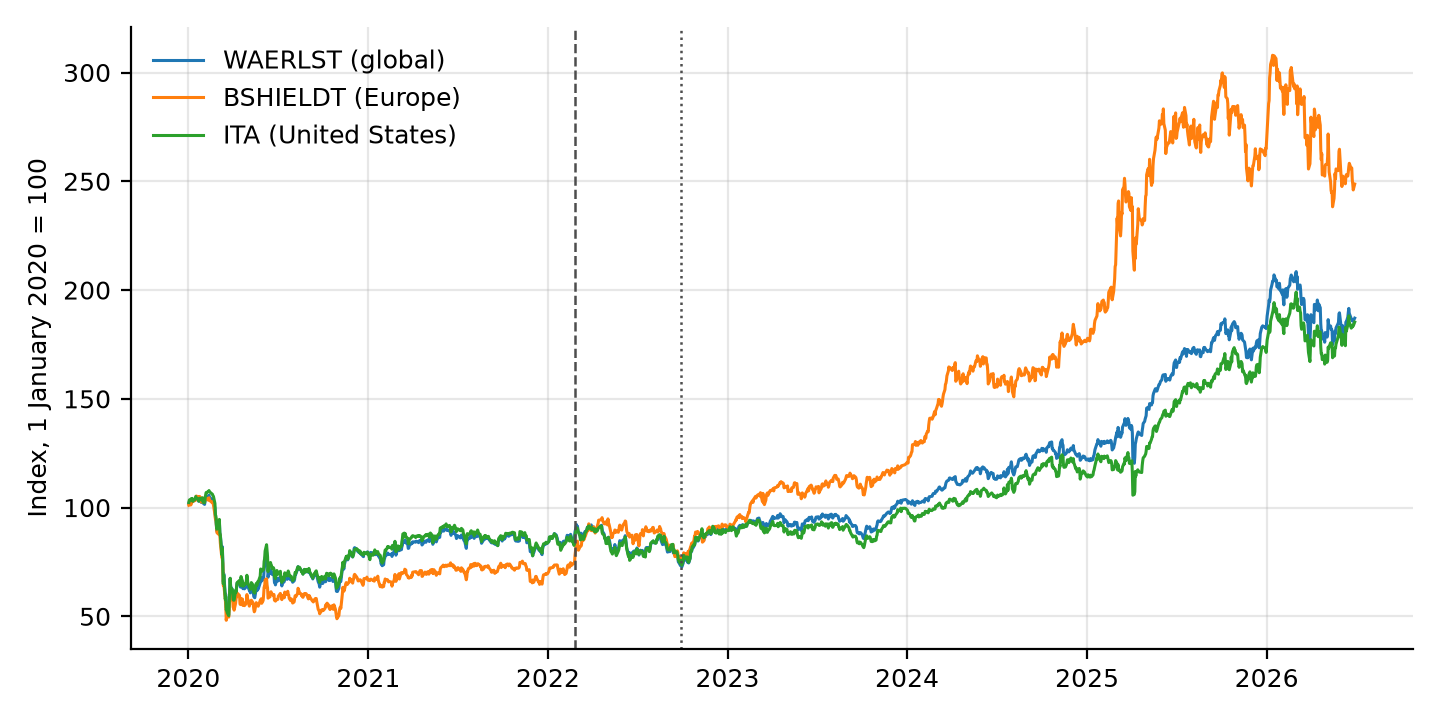
\includegraphics[width=\textwidth]{fig1_defense_indices.png}
\caption{Defence-equity index levels, 1 January 2020 = 100, to June 2026. \textbf{WAERLST} (blue) is the Bloomberg World Aerospace \& Defense Total Return Index; \textbf{BSHIELDT} (orange) is the Bloomberg Europe Defense Select Total Return Index; \textbf{ITA} (green) is the iShares U.S.\ Aerospace \& Defense ETF. The dashed vertical line marks the full-scale invasion (24 February 2022); the dotted vertical line marks 29 September 2022, the first day of the Ukrainian Air Force attack record used in Section~\ref{sec:attacks}. All three series are total-return indices, so the vertical distance between them is cumulative performance including dividends, not a price-only comparison.}
\label{fig:prices}
\end{figure}

\textbf{Figures~\ref{fig:attention} and~\ref{fig:tone} plot the perception indices that are the regressors of interest.} The most striking feature of Figure~\ref{fig:attention} is that the two media environments occupy entirely different levels throughout the eleven years. Ukrainian and Russian outlets devote 71--85\% of their output to conflict-related content on an average day and never fall below 41\%, while Western and native-English outlets average 7.2\% and 5.4\% and stay in single digits until the invasion. This is not two media environments covering the same war at different intensities --- it is two media environments covering different worlds. The invasion is visible as a step change in the Western lines, from 19.0\% on 23 February 2022 to 40.9\% on the 24th, and in the native-English lines, from 11.8\% to 23.8\%. In the same two days Ukrainian attention moves from 90.3\% to 95.8\% and Russian state attention from 84.6\% to 91.2\%: the local ecosystems had almost no room left to react, which is the mechanical reason a Western investor watching coverage volume would have seen a signal in Western outlets and nothing much in local ones.

\begin{figure}[H]
\centering

\includegraphics[width=\textwidth]{fig1_attention_full_sample.png}
\caption{Conflict attention share by media ecosystem, 30-day moving average, 18 February 2015 -- 20 May 2026. Each line shows the share of each ecosystem's daily article output that covers conflict in Ukraine or Russia. Shading marks four war regimes: pre-war (white), build-up (light grey, Nov 2021 -- Feb 2022), invasion (dark grey, Feb -- Jun 2022), and attrition (medium grey, Jul 2022 onward). The dashed vertical line marks 24 February 2022.}
\label{fig:attention}
\end{figure}

Figure~\ref{fig:tone} reveals a striking asymmetry at the invasion. \textbf{Ukrainian conflict tone falls sharply and stays down; Russian state tone barely moves.} Before 2022 the five tone series interleave with no stable ordering; after 24 February 2022 the Ukrainian line separates downward (by $-1.66$ points; see Table~\ref{tab:invasion_tone}) and remains separated for the rest of the sample, while the Russian state line stays within its pre-war band.

\begin{figure}[H]
\centering

\includegraphics[width=\textwidth]{fig2_tone_full_sample.png}
\caption{Mean conflict tone by media ecosystem, 30-day moving average, same sample and regime shading as Figure~\ref{fig:attention}. GDELT tone ranges from $-10$ (most negative) to $+10$ (most positive). Before 2022 the five series interleave with no stable ordering. After 24 February 2022 the Ukrainian line separates downward and stays separated; the Russian state line does not move out of its pre-war band.}
\label{fig:tone}
\end{figure}

\textbf{Russian state media's tone did not change when Russia invaded Ukraine, and Table~\ref{tab:invasion_tone} quantifies how far that is from what every other ecosystem did.} Ukrainian tone falls by 1.66 points, native-English by 0.64, Western by 0.36; Russian state tone moves by $+0.02$, which is to say not at all. The result is not an artefact of which outlets happen to be in the corpus on either side of the invasion: on a fixed panel of the 24 state outlets present in both windows with at least 200 conflict articles in each, the mean shift is $-0.05$. Several state outlets in fact became \textit{more positive} --- \textit{Gazeta.ru} ($+0.48$), \textit{Ren.tv} ($+0.43$), \textit{mskagency.ru} ($+0.40$) --- which is what one would expect from outlets covering the launch of an operation their government had announced as a success. This contrast is the largest and most robust descriptive fact in the data, and it is the reason the pricing null that follows is interesting rather than merely negative: the ecosystem whose signal changed most sharply at the defining event of the sample is not the ecosystem whose signal the market tracks.

\begin{table}[H]
\centering
\caption{Conflict tone before and after the full-scale invasion, by ecosystem}
\label{tab:invasion_tone}
\begin{threeparttable}
\compact
\begin{tabular}{lrrr}
\toprule
Ecosystem & Pre-invasion & Post-invasion & Shift \\
 & (Nov 2021 -- 23 Feb 2022) & (24 Feb -- 5 Jun 2022) & \\
\midrule
Ukrainian (UA) & $-1.77$ & $-3.43$ & $\mathbf{-1.66}$ \\
Native-English (EN\_GLOBAL) & $-1.87$ & $-2.51$ & $-0.64$ \\
Western (WEST) & $-1.90$ & $-2.27$ & $-0.36$ \\
\textbf{Russian state (RU\_STATE)} & $\mathbf{-1.81}$ & $\mathbf{-1.79}$ & $\mathbf{+0.02}$ \\
Russian independent (RU\_INDEP) & $-2.09$ & $-2.01$ & $+0.09$ \\
\bottomrule
\end{tabular}
\begin{tablenotes}
\small
\item Notes: Mean GDELT tone score over the two windows named in the column headings (115 pre-invasion and 102 post-invasion days); more negative values indicate more negative coverage. Ecosystems are ordered by the size of the shift. Produced by \texttt{scripts/make\_thesis\_descriptives.py}.
\item \textbf{The comparison this table is used for is Ukrainian against Russian state, and that contrast is large and robust.} Ukrainian tone falls by 1.66 points; Russian state tone does not move. The Russian state figure is not an artefact of which outlets happen to be in the corpus on each side of the invasion: on a fixed panel of the 24 state outlets present in both windows with at least 200 conflict articles in each, the mean shift is $-0.05$, the same magnitude as the aggregate. A supremum-Wald test for a break at an unknown date, free to choose any day in the interior 70\% of the sample, puts Ukrainian tone's largest break on exactly 24 February 2022, while Russian state tone's largest break falls 393 days later.
\item \textbf{The comparison this table is \textit{not} used for is Russian state against Russian independent.} The two differ by 0.07 points in the aggregate and by 0.11 on the fixed panel, and a formal test of that gap does not reject ($p = 0.561$). An earlier version of this project reported that gap as a ``censorship wedge''; it did not survive correcting the outlet register, and Section~\ref{sec:robustness} records why. The Russian independent block is small --- four outlets clear the fixed-panel threshold, against 24 state outlets --- which is the proximate reason the comparison is underpowered.
\end{tablenotes}
\end{threeparttable}
\end{table}

%==============================================================
\section{Empirical Findings, Interpretation, and Implications}
\label{sec:findings}
%==============================================================

\subsection{Gates 2 and 3: local perception and defence-equity returns}
\label{sec:gate3}

\textbf{Local media add nothing to defence-equity returns that Western media do not already carry, in either of the two forms the question can be asked.} Table~\ref{tab:gates23} reports both. Gate 2 asks it of raw coverage volume and tone --- does the local ecosystem's attention or sentiment move returns? Gate 3 asks it of structure --- does the local split between anticipated and realised conflict, which media at war record very differently from media watching one, move returns? Gate 3 was pre-registered, with its pass rule, its excluded targets and its sign condition fixed in a committed document before the data it uses were collected.

\begin{table}[H]
\centering
\caption{Local-media joint F-tests on defence-equity returns (Gates 2 and 3)}
\label{tab:gates23}
\begin{threeparttable}
\compact
\begin{tabular}{llrrrl}
\toprule
Gate & Block and news timing & Cells & BH survivors & Min.\ $p$ & Verdict \\
\midrule
\multicolumn{6}{l}{\textit{Gate 2: coverage volume and tone}} \\
2 & Local, news lagged 1 day \textit{(primary)} & 31 & 1 & 0.0009 & FAIL \\
2 & Local, same-day & 31 & \textbf{7} & 0.000002 & ---$^{a}$ \\
2 & \textit{Western, news lagged 1 day (control)} & 31 & 0 & 0.0027 & --- \\
2 & \textit{Western, same-day (control)} & 31 & 0 & 0.018 & --- \\
\addlinespace
\multicolumn{6}{l}{\textit{Gate 3: anticipated/realised split (pre-registered)}} \\
3 & Local, news lagged 1 day \textit{(primary arm)} & 31 & 2 & 0.000006 & FAIL$^{b}$ \\
3 & Local, same-day \textit{(secondary arm)} & 31 & 0 & --- & FAIL \\
3 & \textit{Western, news lagged 1 day (control)} & 31 & \textbf{2} & \textbf{0.00016} & PASS \\
\bottomrule
\end{tabular}
\begin{tablenotes}
\small
\item Notes: Each cell is a joint $F$-test on one block of coefficients in equation~(\ref{eq:main}), with the other block, the regional market control and VIX already in the regression; HAC(5) standard errors. The grid crosses daily/weekly frequency, six conflict-episode windows plus the full sample, and five defence-equity targets, giving 31 cells that clear the minimum-observation rule. Benjamini--Hochberg correction at 5\% FDR is applied across all 31 cells of an arm simultaneously. ``Min.\ $p$'' is the smallest uncorrected $p$-value in the arm, reported so that the survivor count can be read against the strength of the strongest single cell. \textbf{Lagged is the primary timing convention}: GDELT days are full UTC days while European markets close at 16:30 UTC, so only news credited to the following trading day was reliably available to trade on.
\item[$a$] \textbf{This row is the informative one, and it is not evidence for local pricing.} Seven of 31 same-day cells survive correction, at a minimum $p$ of $2\times10^{-6}$ --- so the design is emphatically able to detect the local block when the local block is there to detect. Crediting the same news to the next trading day, which removes only the portion published after the European close, reduces those seven survivors to one. Information the market had not yet impounded should have survived that shift; what does not survive it is the mechanical same-day association that efficient pricing predicts.
\item[$b$] The two Gate 3 primary survivors are both weekly and both in the 2025--26 episode window (58 observations against 13 parameters). The two deepest cells in the grid, the pooled daily specifications with 2,754 observations each, return $p = 0.08$ and $p = 0.36$. Neither pre-registered arm clears: Arm 1 requires a surviving cell in the Russia build-up window on a Bloomberg target or ITA, and on the corrected register that window produces no surviving cell at all (smallest $p$ there is 0.018); Arm 2 requires same-sign survivors in two independent episode windows, and the two that survive share a window.
\end{tablenotes}
\end{threeparttable}
\end{table}

\textbf{The timing contrast in Gate 2 is the most informative single result in this thesis, and it is what rules out the low-power explanation of the null.} Local coverage is strongly associated with defence returns when it is credited to the day it was published: seven of 31 cells survive correction, the strongest at $p = 2\times10^{-6}$. Credit the same coverage to the next trading day --- the only convention under which a trader could actually have used it, since GDELT days run to midnight UTC and European markets close at 16:30 --- and seven survivors become one. The lag removes only the news published after the close. Genuine unimpounded information should therefore have survived it almost intact; a mechanical contemporaneous association should not. What survives is the pattern efficient pricing predicts, and running only one of the two alignments would have made the two indistinguishable.

\textbf{Gate 3 reaches the same verdict on the structural version of the question, and its two survivors fail the pre-registered rule for a reason worth stating.} They are both weekly cells in the 2025--26 episode window, fitting 13 parameters to 58 observations, while the two deepest cells in the grid --- pooled daily specifications with 2,754 observations each --- return $p = 0.08$ and $p = 0.36$. An effect that concentrates in the thinnest corner of a grid and disappears where the data are deepest is the signature of noise rather than of a small true effect awaiting more power. The Western block, tested in the same 31 cells under the same correction, does survive, at a minimum $p$ of 0.00016. That asymmetry --- Western detected, local not, in identical cells --- is the finding.

\textbf{Gate 3 also contained a seductive sign pattern.} Among the surviving weekly cells, coefficients showed consistent ``buy the rumour, sell the fact'' signs in Ukrainian media: a shift toward anticipatory coverage raised defence returns, a shift toward realised conflict lowered them. Those four signs were written down and tested on the 2017--19 window that had not been seen when the hypothesis was formed: 7 of 12 signs matched (binomial p = 0.387). The pattern was in-sample noise. This episode is the clearest illustration that pre-registered tests on partial samples are not genuinely pre-registered.

\subsection{Gates 4 and 5: gas and escalation}
\label{sec:gates45}

\textbf{Gates 4 and 5 move the test to the two outcomes where local information should matter most, and the null survives both.} If the defence-equity result were an artefact of defence equities being a poor testbed --- which is a fair objection, since the link from a Russian newspaper to a U.S.\ contractor's share price runs entirely through Western investors --- then it should break on an asset with a direct physical transmission channel, or on an outcome with no market in it at all. Table~\ref{tab:gates45} tests both. European natural gas is the asset through which the conflict physically transmitted to Europe (Russia supplied $\sim$40\% of EU gas; TTF rose from $\sim$\euro{}20 to $\sim$\euro{}300); realised escalation is the war outcome itself. Both tests were pre-registered before their data were ingested.

\begin{table}[H]
\centering
\caption{Local-media joint tests on European gas (Gate 4) and realised escalation (Gate 5)}
\label{tab:gates45}
\begin{threeparttable}
\compact
\begin{tabular}{llrr}
\toprule
Gate / Window & $n$ & $p$ (local block) & $p$ (Western block) \\
\midrule
\multicolumn{4}{l}{\textit{Gate 4: Dutch TTF natural gas, daily returns}} \\
(a) Build-up and invasion, Jun 2021 -- Jun 2022 & 222 & 0.399 & \textbf{0.00004} \\
(b) Shutdown and aftermath, Jun 2022 -- Jun 2023 & 231 & 0.533 & 0.193 \\
(c) Full crisis, Jun 2021 -- Dec 2023 & 563 & 0.250 & 0.066 \\
\addlinespace
\multicolumn{4}{l}{\textit{Gate 5: realised escalation (GPR\_ACT), held-out sample}} \\
Horizon $h=1$ day & 637 & 0.212 & 0.171 \\
Horizon $h=5$ days & 629 & 0.227 & \textbf{0.033} \\
\bottomrule
\end{tabular}
\begin{tablenotes}
\small
\item Notes: Each entry is the $p$-value of a joint $F$-test on one block --- local (Ukrainian, Russian state, Russian independent attention and tone changes) or Western --- with the other block and the controls already in the regression; HAC(5) standard errors. Bold marks $p<0.05$. Gate 4 regresses daily TTF returns; Gate 5 regresses the realised-conflict component of the \citet{caldara2022} index on 637 held-out days that were never used in sample. Both tests were pre-registered, and in both cases the data were ingested after the pre-registration was committed, which is verifiable from the repository history.
\item \textbf{All four of Gate 4's pre-registered conditions fail}, and they fail in different ways, which is what makes the verdict robust rather than marginal: no BH survivor in either required window; the placebo condition breached, since local perception ``explains'' Brent crude ($p = 0.0014$) as readily as European gas; the build-up result does not survive dropping the ten largest TTF moves ($0.399 \rightarrow 0.840$); and the ordering is wrong, with Russian \textit{independent} rather than Russian \textit{state} media leading the local block, which inverts the supply-signalling mechanism the test was built to detect.
\item \textbf{The Western block behaves differently in the two gates, and the honest reading is that Gate 4 carries the positive control and Gate 5 carries it only weakly.} In Gate 4's build-up window the Western block is detected at $p = 4\times10^{-5}$ in the same specification where the local block returns 0.399 --- the sharpest positive control anywhere in this thesis. In Gate 5 the Western block is significant at the five-day horizon ($p = 0.033$) but not at one day ($p = 0.171$), so Gate 5 on its own would not establish that the design has power; it is reported as corroboration, not as an independent control. A shuffle placebo returns $p = 0.557$ and $0.799$, confirming the procedure does not manufacture significance from noise.
\end{tablenotes}
\end{threeparttable}
\end{table}

\textbf{Gate 4 shows that the null is not a property of defence equities being a weak testbed.} European gas is the asset where Russian supply signals should matter most --- Russia supplied roughly 40\% of EU gas and TTF moved from about \euro{}20 to over \euro{}300 --- and Russian state media is the channel through which supply intent was signalled. Yet the local block returns $p = 0.399$ in the build-up window, and all four pre-registered conditions fail. In the same specification the Western block is detected at $p = 4\times10^{-5}$, which is the clearest demonstration in this thesis that the apparatus finds effects where they exist.

\textbf{Gate 4 is also this project's clearest illustration of how a positive can appear and then dissolve under replication.} The exploratory version of this test, run on the 81 days of build-up coverage that had been ingested at the time, returned $p = 0.0028$ under the same controls the confirmatory run would use, and $p = 0.002$ under a slightly different set --- a result stable enough across control choices to look robust. The pre-registered confirmatory run, on the same asset, the same specification, the same controls and the same calendar period, with nothing changed but the quantity of data, returned $p = 0.399$ on 222 continuous days. The result was not overturned by a better control or a stricter correction. It was overturned by more of the data it had always been about, which is the failure mode that pre-registration exists to expose.

\textbf{Gate 5 removes prices from the test entirely and asks whether local perception anticipates the war's own escalation.} If local media carry genuine information about the conflict, they should at minimum lead a measure of realised conflict, whether or not any asset prices it. On 637 held-out days never used in sample they do not: the local block returns $p = 0.21$ at one day and $p = 0.23$ at five, and does not survive twelve lags of the outcome's own dynamics. This gate is weaker evidence than the other three, because its own Western control is significant at five days ($p = 0.033$) but not at one ($p = 0.171$); it is reported because a pre-registered test must be reported whatever it returns, and because a null on a non-market outcome closes the escape route that the earlier nulls are all artefacts of market microstructure.

\subsection{Out-of-sample predictability}
\label{sec:efficiency}

\textbf{Nothing in the preceding tests is a claim about forecasting, and this section supplies the forecasting test the supervisor's review asked for.} A contemporaneous association can exist without being usable, and a null on contemporaneous association does not by itself establish that a trader could not have profited; the two questions need separate evidence. Table~\ref{tab:efficiency_power} reports the out-of-sample results together with the power simulation that makes their null interpretable. The forecasting grid has five targets and ten predictors (attention share and tone for each of five ecosystems), giving 50 specifications. The Clark--West test \citep{clark2007} arbitrates each. Where models are non-nested, the Diebold--Mariano test \citep{diebold1995} with the Harvey--Leybourne--Newbold small-sample correction \citep{harvey1997} is used instead.

\begin{table}[H]
\centering
\caption{Out-of-sample return predictability and test power}
\label{tab:efficiency_power}
\begin{threeparttable}
\compact
\begin{tabular}{lr}
\toprule
\multicolumn{2}{l}{\textit{Panel A: Clark--West results across the full grid}} \\
\midrule
Specifications (5 targets $\times$ 10 predictors) & 50 \\
Out-of-sample days per specification & 1,855 or 686 \\
Positive Campbell--Thompson R$^2_{\text{OS}}$ & 3 of 50 \\
Best R$^2_{\text{OS}}$ observed & $+0.0010$ \quad ($+0.10\%$) \\
Smallest Clark--West $p$-value & 0.067 \\
Clark--West $p < 0.05$ & \textbf{0} \quad (2.5 expected by chance) \\
Survive Benjamini--Hochberg (5\% FDR) & \textbf{0} \\
\midrule
\multicolumn{2}{l}{\textit{Panel B: Simulated power, 1,855 OOS days, 60 paths per row}} \\
\midrule
True R$^2_{\text{OS}}$ = 0.0\% (nominal size) & 0.02 \\
True R$^2_{\text{OS}}$ = 0.2\% & 0.47 \\
True R$^2_{\text{OS}}$ = \textbf{0.5\%} & \textbf{0.83} \\
True R$^2_{\text{OS}}$ = 1.0\% & 1.00 \\
True R$^2_{\text{OS}}$ = 2.0\% & 1.00 \\
\bottomrule
\end{tabular}
\begin{tablenotes}
\small
\item Notes: Expanding-window, one-day-ahead design with a minimum 250-day training window, re-estimated at each step. Each specification adds one perception predictor --- the lagged daily change in attention share or tone for one ecosystem --- to a historical-mean benchmark. Because setting that predictor's coefficient to zero returns the benchmark exactly, the comparison is nested and is arbitrated by the Clark--West test \citep{clark2007} with a Bartlett long-run variance estimator, one-sided in the direction of model improvement. Out-of-sample length differs by target: the three free-data targets yield 1,855 out-of-sample days each and the two Bloomberg indices, which begin in 2020, yield 686.
\item Panel B simulates power by implanting a predictor with a known true R$^2_{\text{OS}}$ into the actual return series and running the identical expanding-window machinery over 1,855 out-of-sample days. \textbf{The simulation uses 60 paths per row, so each rejection rate carries a standard error of roughly six percentage points}; the entries should be read as locating the power curve, not as precise to the second decimal. Nominal size in the first row is 0.02 against a nominal 5\%, confirming the test is conservative rather than over-rejecting --- which means the null in Panel A is not produced by a test that cannot reject.
\end{tablenotes}
\end{threeparttable}
\end{table}

\textbf{Zero Clark--West rejections across 50 specifications is a bound, not an absence.} Panel B quantifies what the null rules out. The 0.5--1.0\% range of out-of-sample R$^2$ that \citet{welch2008} and \citet{campbell2008} treat as the threshold for economic significance is detected in 83\% of simulated samples at the bottom of that range and in all of them at the top. The best value actually observed, $+0.10\%$, sits below even the 0.2\% effect size that the design detects only about half the time --- and its Clark--West $p$-value is 0.067, so not one of the fifty specifications reaches nominal significance, let alone survives correction. What can be claimed is therefore bounded in both directions: an effect large enough to matter economically would very probably have been seen, and an effect small enough to have escaped this design is too small to trade.

\subsection{Discussion: what this null means}
\label{sec:robustness}

\textbf{The null is consistent across all four tests and both asset classes.} Local perception adds nothing in volume, in tone, in the threat/act structure, in the most natural testbed (gas), in the most demanding outcome (escalation itself), or out of sample. The Western block survives correction as a positive control in three of the four gates --- the anticipation gate, gas, and escalation --- and the fourth gate is sensitive in a different and more informative way, since it is there that the local block's own same-day detections collapse under the tradeable lag. This co-occurrence --- local block null, Western block or timing structure detected, in the same cells --- is the result. It says that the design can measure the effect of media on prices; it measures Western media and finds an effect; it measures local media and does not.

\textbf{Western investors respond to the signal that moved, and the descriptive chapter shows which signal that was.} Russian state media's tone did not change when Russia invaded Ukraine, and Ukrainian and Russian attention were already near saturation and had almost no room to rise. Western attention, by contrast, doubled in a day. If the marginal buyers and sellers of Western defence equities form their views from Western coverage --- which is what the null says --- then they responded to the one series in the data that registered the event. The information asymmetry between the two media environments is real and large; what does not follow is that the asymmetry advantages local media from the standpoint of a Western investor. Coverage that is already saturated cannot rise when something happens, and a signal that does not move cannot move a price.

\textbf{The result was not the prior, and the direction in which it disappoints is worth stating.} The design was built expecting to find something. Local media are closer to the events, cover them earlier and in far greater volume, and \citet{bondarenko2024} had already shown local-language risk measures carrying information that English-language ones did not. The pre-registrations were written to catch a positive, and Gates 4 and 5 were added specifically because defence equities are a weak testbed --- an objection this thesis raised against itself before an examiner could. The prior was that local perception would add \textit{something}, most plausibly in the anticipation structure of Gate 3. It did not.

\textbf{Reconciling that with the literature requires being precise about what \citet{bondarenko2024} actually established.} Their finding is that local-language geopolitical-risk shocks move the \textit{Russian} economy while English-language shocks do not. The natural extrapolation --- local sources are simply better measures of geopolitical risk --- is the one this thesis rejects. What survives is narrower and more useful: the informative ecosystem is the one inhabited by the agents whose decisions are being measured. Russian firms and households read Russian newspapers, so Russian coverage moves Russian output; Western fund managers read Western newspapers, so Western coverage moves Western defence equities. Read that way the two results are not in tension at all, and neither is a claim about which journalists are better informed.

\textbf{The result also refines, rather than contradicts, the defence-equity event-study literature.} \citet{apergis2018defense}, \citet{zhang2022race}, \citet{covachev2024europe} and \citet{klomp2025hamas} all document defence equities responding to conflict news, and nothing here disputes that: the Western block is detected in the pre-registered anticipation gate and in the gas test. What this thesis adds is that the response is specific to the Western reporting layer rather than to conflict news as such. That distinction is invisible to a design that aggregates coverage without regard to the publisher, which is what every one of those studies does --- and it is invisible for a reason worth noting, since separating publishers requires a translingual corpus that only became available part-way through the period they study.

\textbf{The physical record of the war does not forecast defence-equity returns either, which closes off the reading that the news measures are simply a poor proxy for the war itself.} On the September 2022 -- June 2026 subsample where the Ukrainian Air Force attack data exist, 144 specifications race five information sets --- physical attacks alone, news alone, and their combinations --- against historical-mean and AR(1) benchmarks across three targets, two horizons and two samples. Sixteen achieve a positive out-of-sample R$^2$ and \textbf{none survives Benjamini--Hochberg correction}; the benchmarks win the majority of cells outright. Knowing how many missiles were launched yesterday does not help predict what defence equities do today, any more than knowing what was written about them does.

\textbf{Nor do war signals forecast defence-equity volatility, which is the arm where a positive result was most plausible.} Returns are hard to forecast even in principle, but volatility is persistent and forecastable, so if conflict news carried usable information this is where it should appear. Forty-eight augmented HAR-RV-X specifications \citep{corsi2009} are evaluated against GARCH, GJR-GARCH and EGARCH benchmarks under the QLIKE loss. \textbf{None is significantly better than its benchmark; eight are significantly worse}, and all six specifications that survive multiple-testing correction are deteriorations rather than improvements. Adding war variables to a volatility model makes it worse. Both of these exercises are exploratory rather than pre-registered, and are reported as such.

\textbf{Six results that were significant when found did not survive, and the six failure modes are all different.} Two fell to an omitted variable: a defence-volatility result and a build-up threat-shock result, both of which used the S\&P 500 as the market control for European defence equities and both of which vanished when the STOXX 600 replaced it (the second moving from $p = 0.0001$ to $p = 0.84$). One fell to a truncated sample: Gate 3 passed on the data ingested at the time and failed once the held-out window was added, seven survivors becoming two. One fell to pre-registered replication on more data: the gas result, $p = 0.0028$ on 81 days and $p = 0.399$ on 222 days of the same period. One fell to out-of-sample testing: an escalation result significant in both halves of the in-sample period and $p = 0.21$ on the held-out window. And one fell to a composition change: the state-versus-independent tone wedge, which rested on outlets misfiled into the Russian independent register --- Deutsche Welle among them --- and which moved \textit{further} from significance with each successive correction to that register, ending at $p = 0.561$.

\textbf{The pattern across those six is the reason to believe the null.} Each was significant at conventional levels. Each had a mechanism that could be told as a story. Each survived at least one robustness check before failing another. Two were killed by better controls, one by more data, one by a test written down before the data existed, one by holding data back, and one by fixing a classification error. A project that ran only the first of any of these pairs would have reported a positive result in good faith. The sequence is documented here rather than suppressed because it is more useful to a researcher entering this literature than an additional coefficient would have been --- and because the null this thesis reports was not obtained by failing to look.

%==============================================================
\section{Conclusion}
%==============================================================

\textbf{The Western narrative is what is priced in Western defence equities.} Local-language perception of the Russia--Ukraine war --- from Ukrainian outlets, Russian state media, and Russian independent outlets --- adds no explanatory power to defence returns conditional on Western coverage, in any of four tests, across two asset classes, and against one non-market outcome. The positive control survives multiple-testing correction in three of the four gates, and in the fourth the local block is itself detected on the day of publication and lost when it is lagged by one day --- so in no gate is the null attributable to a design that cannot see anything. A power simulation on 1,855 out-of-sample days establishes that effects in the range the predictability literature treats as economically meaningful would have been detected in 83\% to 100\% of simulated samples. They were not found.

This result is the mirror image of \citet{bondarenko2024}: their local-versus-English asymmetry runs in the opposite direction for the other side of the conflict. For the Russian domestic economy the local narrative dominates; for Western defence equities the Western narrative dominates. Neither result is a general claim about whether local media matter; together they say that each market prices the information ecosystem that is closest to its own participants.

\textbf{There is a practical implication, and it is the reason a reader with no interest in this particular war should care.} Multilingual geopolitical-risk products are sold on the premise that sources closer to an event carry information that Anglophone coverage misses. This thesis tests that premise where it should hold most strongly and finds that it does not: building a Ukrainian or Russian-language risk index in order to trade Western defence equities is effort spent on a signal the market has already, or has never, priced. The premise is not refuted in general --- \citet{bondarenko2024} show it holding for the Russian domestic economy --- but it cannot be assumed. Whether local sources add anything is an empirical question about the distance between an information ecosystem and a market's marginal investor, and it has to be asked one market at a time.

\textbf{Three limitations bound what this thesis can claim.} The first is that the analysis is associational rather than causal: coverage and prices respond to the same underlying events, and the conditional design separates ecosystems from one another but does not identify a causal effect of coverage on prices. The second is measurement: GDELT tone is a dictionary-based score, and \citet{loughran2011textual} give good reason to treat such scores as indicators of coverage negativity rather than of investor belief; multilingual transformer models applied to article text would sharpen the signal, though they would not change the classification question this thesis is about. The third is frequency: at daily resolution a reaction completed within the trading day is invisible, and the Gate 2 timing result --- which turns on a one-day lag --- is precisely the kind of finding that intraday data could either sharpen or overturn.

\textbf{One limitation the reader might expect is not one.} A natural objection to an index-level null is that it could mask a cross-sectional effect, with heavily war-exposed firms responding where a diversified index does not. That was testable and was tested: a firm-level panel of 31 defence names and 85,065 firm-days, with exposure measured from public SIPRI arms-revenue data, produces no exposure gradient in any war window --- nominal significance appears only in the pre-war period and in a full sample that is 59\% pre-war, and none of the ten cells survives correction. The index-level result is not an aggregation artefact.

\textbf{The most valuable extension is the one that would settle whether this result is general.} Running the same ecosystem comparison on other conflicts --- Hamas--Israel, the Taiwan Strait --- would establish whether the local-versus-Western asymmetry is a property of defence-equity pricing or a feature of this particular war, in which the local-language ecosystems happened to be at coverage saturation before the defining event occurred. A second extension would move to intraday prices, where the anticipation-versus-realisation distinction that Gate 3 could not resolve at daily frequency becomes observable. A third would carry the design to assets whose marginal investors are not Western --- rouble-denominated instruments, or the sovereign debt of states bordering the conflict --- which is the sharpest available test of the claim that each market prices the ecosystem its own participants inhabit.

\newpage
\bibliography{references}

\end{document}
